% -*- coding: utf-8 -*-

\section{TreeBoost}
% http://nbviewer.jupyter.org/github/facaiy/book_notes/blob/master/machine_learning/tree/gbdt/treeboost/intro.ipynb
\subsection{直观印象}
% 全局权重 -> 叶子权重
\begin{frame}
    \begin{align*}
        \mathbf{a}_m &= \operatorname{arg \, min}_{\mathbf{a}, \beta} \textstyle \sum_{i=1}^N \left [ \tilde{y}_i - \beta h(x_i; \mathbf{a}) \right ]^2 \\
        \rho_m &= \operatorname{arg \, min}_\rho \textstyle \sum_{i=1}^N L \left ( y_i, F_{m-1}(x_i) + \rho h(x_i; \mathbf{a}_m) \right)
    \end{align*}

    \begin{figure}
        \centering
        \resizebox{\onepicwidth}{!}{\chapter{前言}
hi!
}
        \caption{Tree boost示意\footnote{
                 \href{http://www.texample.net/tikz/examples/red-black-tree/}{Red-black tree, Madit}}}
    \end{figure}
\end{frame}


\subsection{算法推导}
% 对树建模,公式推导
%% 叶子区域
\begin{frame}{J-叶子树模型}
    $h(x; \{b_j, R_j\}_1^J) = \sum_{j=1}^J b_j \, \mathbf{1}(x \in R_j)$

    \begin{figure}[!tb]
        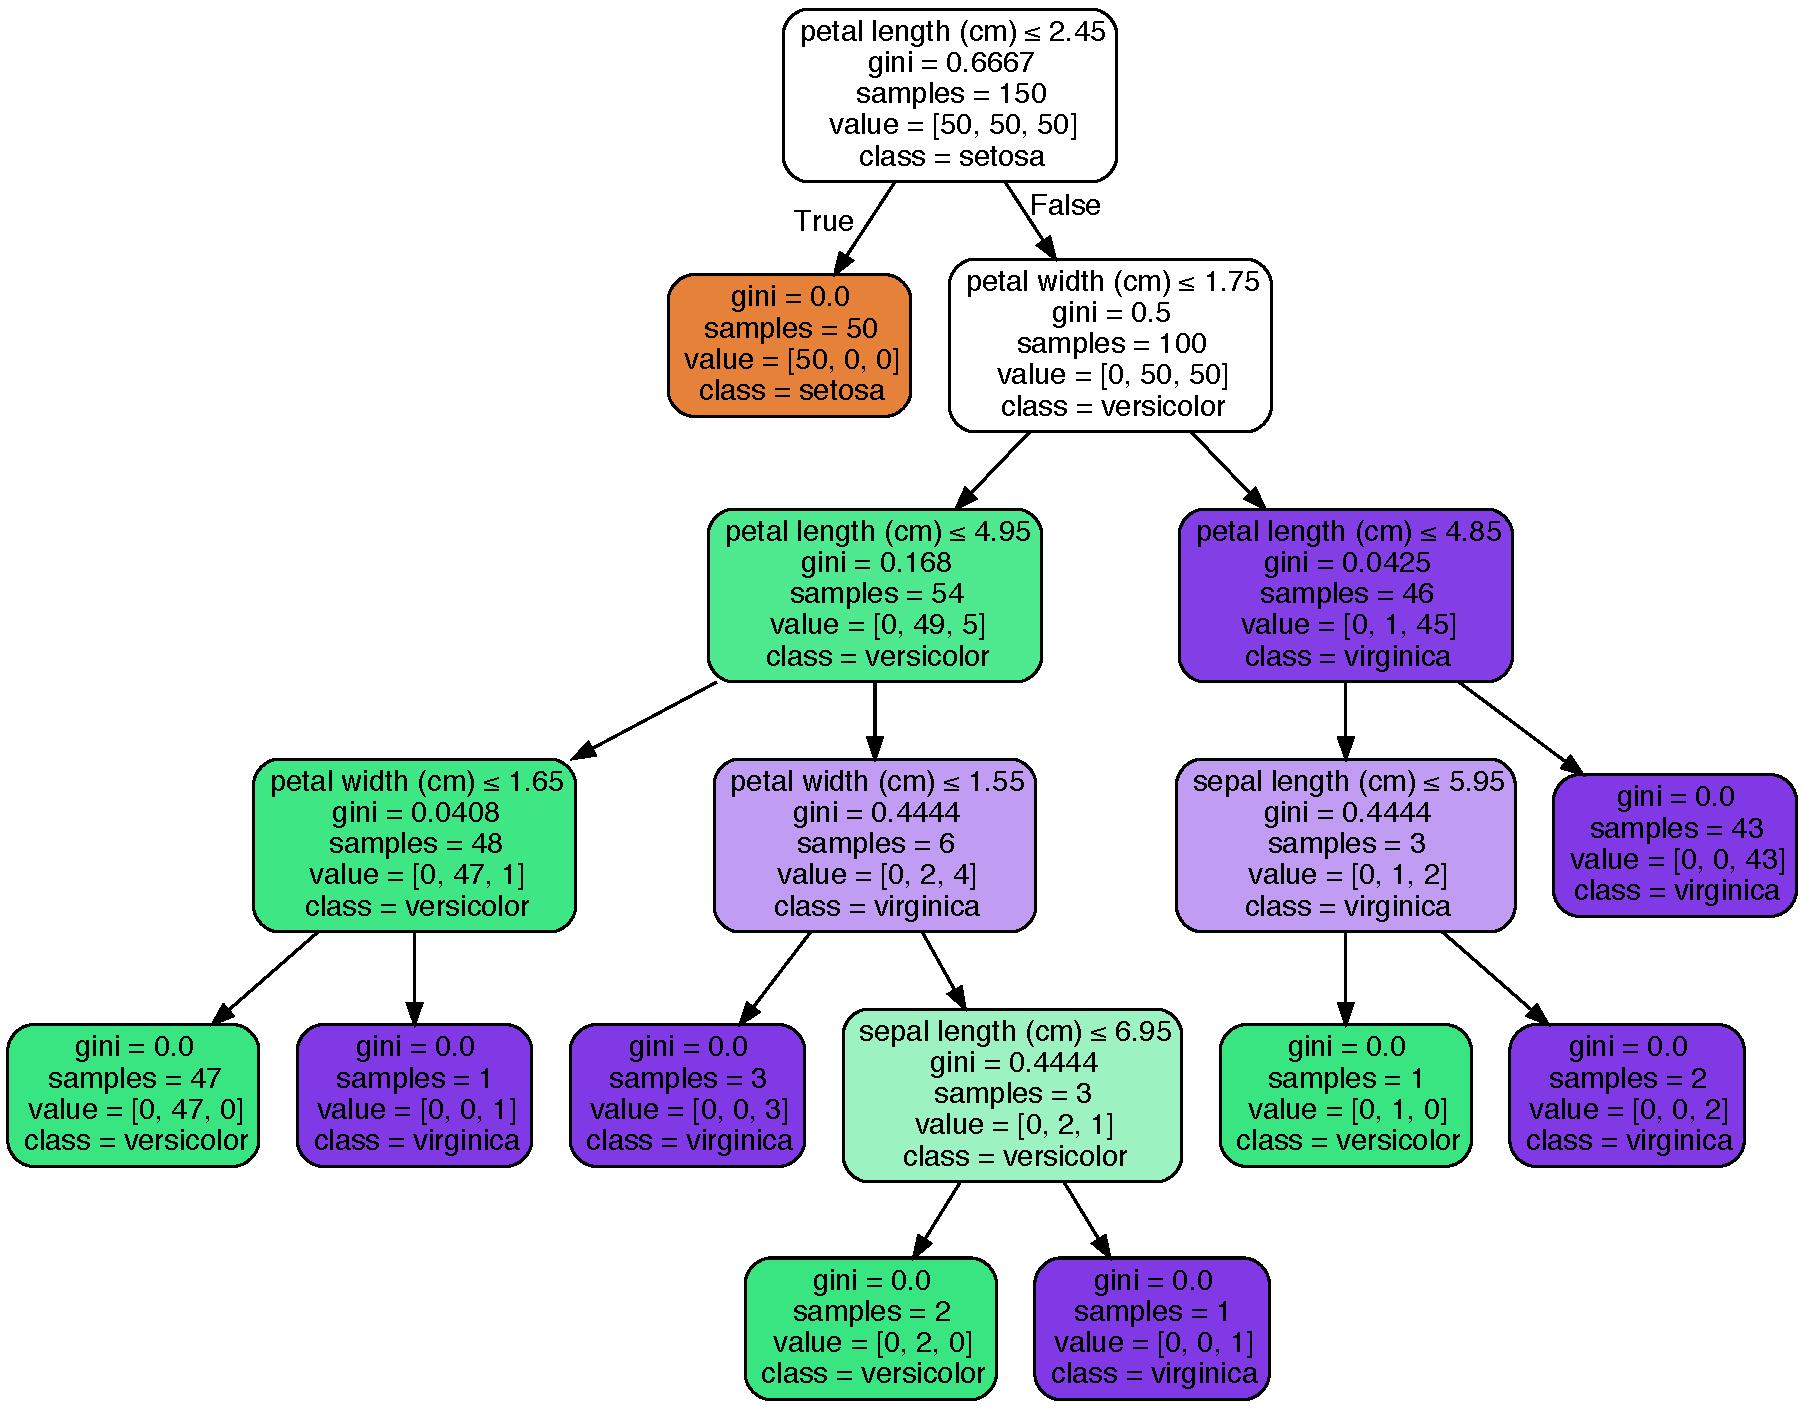
\includegraphics[width=\twopicwidth]{figure/decision_tree/iris}
    \end{figure}
\end{frame}

\begin{frame}
    \begin{align*}
        \rho_m & = \operatorname{arg \, min}_\rho \textstyle \sum_{i=1}^N L \left ( y_i, F_{m-1}(x_i) + \rho h(x_i; \mathbf{a}_m) \right) \\
               & = \operatorname{arg \, min}_\rho \textstyle \sum_{i=1}^N L \left ( y_i, F_{m-1}(x_i) + \rho \sum_{j=1}^J b_j \, \mathbf{1}(x \in R_j) \right) \\
               & = \operatorname{arg \, min}_\rho \textstyle \sum_{i=1}^N L \left ( y_i, F_{m-1}(x_i) + \sum_{j=1}^J \textcolor{blue}{\rho b_j} \, \mathbf{1}(x \in R_j) \right) \\[2ex]
        \{\gamma_{jm}\}_1^J &= \operatorname{arg \, min}_{\{\gamma_j\}_1^J} \textstyle \sum_{i=1}^N L \left ( y_i, F_{m-1}(x_i) + \sum_{j=1}^J \textcolor{blue}{\gamma_j} \mathbf{1}(x \in R_{jm}) \right ) \\[2ex]
        \gamma_{jm} &= \operatorname{arg \, min}_{\gamma} \textstyle \sum_{x_i \in R_{jm}} L(y_i, F_{m-1}(x_i) + \gamma) \\
    \end{align*}
\end{frame}


\subsection{常见的损失函数}
% LS_Boost
%% 残差的来源
%% spark, gbdt, 没有寻优的原因

% LAD_Boost
%% median 不要写公式

% other
%% M_Regression
%% Two_class logistic regression and classification

% 罗列spark和sklearn支持的loss function
\begin{frame}
    $\gamma_{jm} = \operatorname{arg \, min}_{\gamma} \sum_{x_i \in R_{jm}} L(y_i, F_{m-1}(x_i) + \gamma)$

    \vfill

    \begin{block}{L2}
        \begin{align*}
            \gamma_{jm} &= \operatorname{arg \, min}_{\gamma} \sum_{x_i \in R_{jm}} (y_i, F_{m-1}(x_i) + \gamma)^2 \\
                        &= \operatorname{Ave} (y - F_{m-1}(x))
        \end{align*}
    \end{block}

    \begin{block}{L1}
        \begin{equation*}
            \gamma_{jm} = \operatorname{median}_W \left \{ \frac{y_i - F_{m-1}(x_i)}{h(x_i; \mathbf{a}_m)} \right \}_1^N
        \end{equation*}
    \end{block}
%        \item [M-regression] \begin{equation*} L(y, F) = \begin{cases}
%                                    \frac{1}{2} (y - F)^2 \quad & |y - F| \leq \delta \\
%                                    \delta \cdot \left (\big |y - F \big | - \frac{\delta}{2} \right ) \quad & |y - F| > \delta
%                                \end{cases}
%                            \end{equation*}
%        \item [Binary Class] $\gamma_{jm} = \sum_{x_i \in R_{jm}} \tilde{y}_i \Big / \sum_{x_i \in R_{jm}} |\tilde{y}_i| (2 - |\tilde{y}_i|)$
    {\tiny
    详细推导可见:\href{http://nbviewer.jupyter.org/github/facaiy/book_notes/blob/master/machine_learning/tree/gbdt/treeboost/intro.ipynb}{TreeBoost原理和实现(sklearn)简介,颜发才}}
\end{frame}


\subsection{sklearn实现代码}
%\begin{frame}
%    \begin{block}{优点}
%        \begin{itemize}
%            \item 权重更细粒度
%            \item 省去寻优,计算加速
%            \item 实现简单
%        \end{itemize}
%    \end{block}
%%% 损失 + 树 -> 树 == 先验 + 数据 -> 后验
%\end{frame}

\begin{frame}[fragile]
    \begin{lstlisting}[language=Python,style=myScalastyle]
    y_pred = self._decision_function(X)

    def _fit_stage(self, i, X, y, y_pred, sample_weight, sample_mask,
                   random_state, X_idx_sorted, X_csc=None, X_csr=None):
        for k in range(loss.K):
            if loss.is_multi_class:
                y = np.array(original_y == k, dtype=np.float64)

            residual = loss.negative_gradient(y, y_pred, k=k,
                                              sample_weight=sample_weight)
            tree = DecisionTreeRegressor(
                criterion='friedman_mse',
                splitter='best',
                presort=self.presort)

                tree.fit(X_csc, residual, sample_weight=sample_weight,
                         check_input=False, X_idx_sorted=X_idx_sorted)
            # update tree leaves
                loss.update_terminal_regions(tree.tree_, X, y, residual, y_pred,
                                             sample_weight, sample_mask,
                                             self.learning_rate, k=k)
            self.estimators_[i, k] = tree
        return y_pred
    \end{lstlisting}
    {\tiny \tt
    source: scikit-learn/sklearn/ensemble/gradient\_boosting.py \\[-2ex]
    commit: d161bfaa1a42da75f4940464f7f1c524ef53484f}
\end{frame}
